
\section{The Visualisation Module}
\label{sec:the_visualisation_module}

The VisualisationModule class is responsible for showing the current state of the environment, and the vehicles in it, in an appealing and realistic fashion.

To do so, the Visualisation Module opens up a Visualisation Window, where the user can get a bird's eye view of the environment, that is updated in real time. This module relies heavily on Python's graphical library pygame.

The Visualisation Module interfaces with the SML World through the use of UDP communications, implemented in the auxiliary classes VisualisationModuleSender and VisualisationModuleReceiver.

\subsection{The Visualisation Module}

The objective of the Visualisation Module is to show to the user, the environment in a Visualisation Window. Unlike other Modules, the Visualisation Module runs independently (\textit{i.e.}, in a completely independent thread, see \ref{visualisation_module:threading_restrictions}) from the SML World. Image \ref{fig:visualisation_module_diagram} shows a diagram representing its structure.

\begin{figure}[h!]
  \centering
    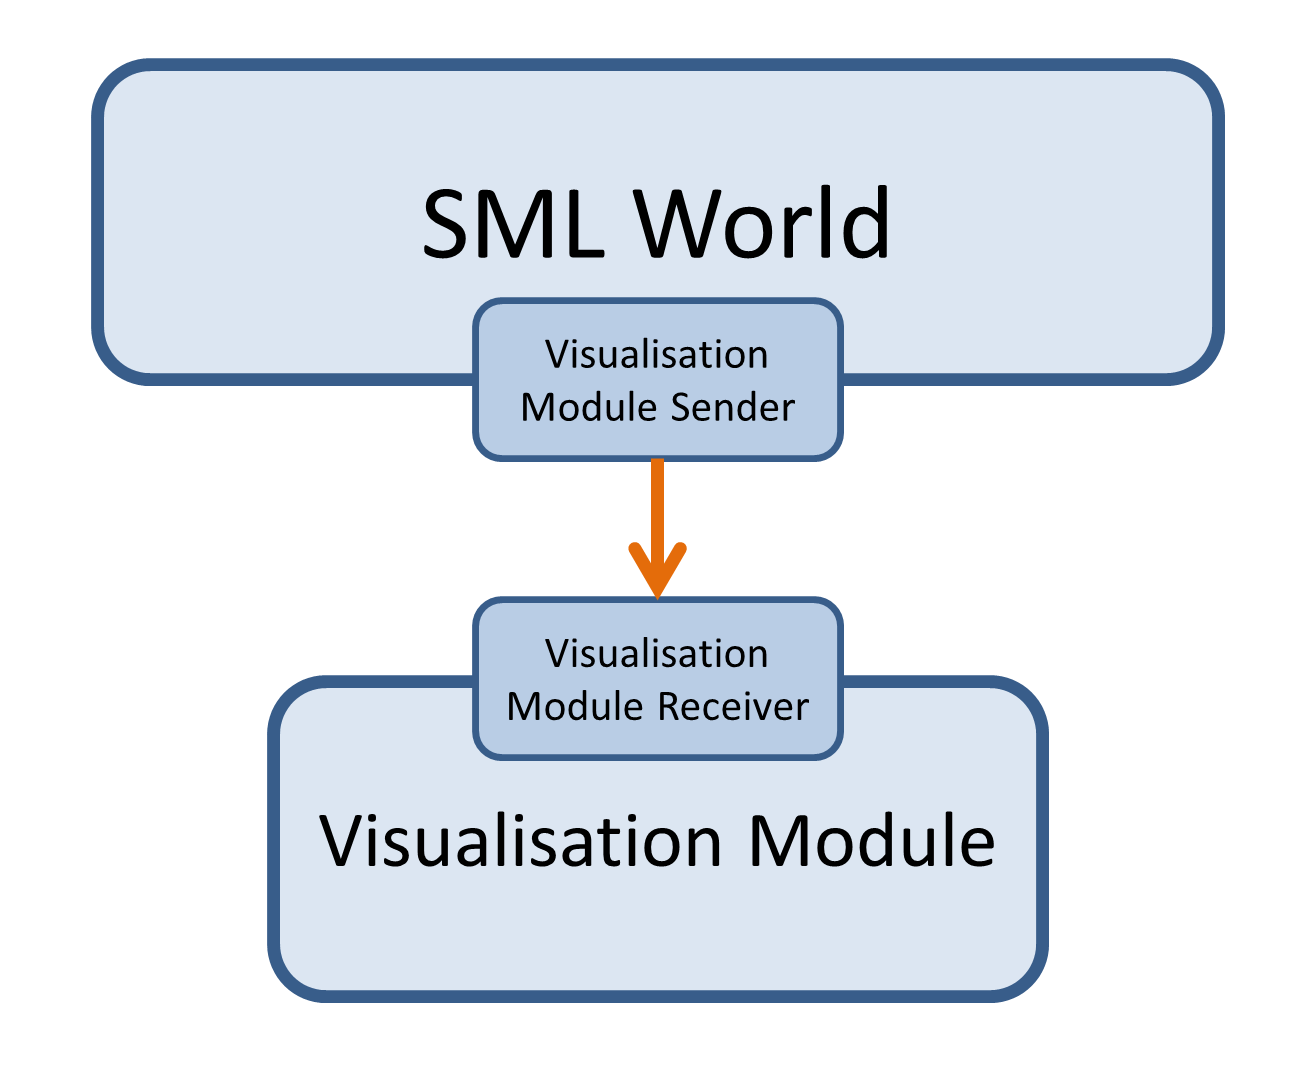
\includegraphics[width=0.6\textwidth]{visualisation_module_diagram}
    \caption{Diagram of the Visualisation Module interfacing with the SML World \label{fig:visualisation_module_diagram} }
\end{figure}

The SML World and Visualisation Module interface with each other using the auxiliary classes VisualisationModuleSender and VisualisationModuleReceiver. These classes establish a one-way UDP communication from the SML World to the Visualisation Module. The information transmitted over this communication link consists of the current vehicle states in the SML World.

\subsubsection{Loading the Environment Information}

The first step of the Visualisation Module is to load the environment information. This corresponds to the image depicting the environment, and the properties of this image.

To do so, the class constructor receives an argument \texttt{map\_filename}. This corresponds to a string with the location and name of the image to be loaded. This string must not have the extension of the image in it, since we will simply use the name of the image to fetch, both the image, and the metadata associated with the image. The image is simply obtained by appending the bitmap image extension (\texttt{map\_filename + .bmp}). The metadata of the image can be found as \texttt{map\_filename + .meta}.

The metadata file contains information about the image size, width and height, and the ration of pixels per meter. This information is necessary in order to know where in the image the vehicles should be drawn, given their Cartesian coordinates.

\subsubsection{From Meters To Pixel}

An important step in the Visualisation Tool, is to know where to draw the vehicles. Or in more simple terms, if I have a vehicle at cartesian coordinates $(x, y)$, what is the corresponding pixel position? To do so we need to define our meters to pixel converter function.

By default, all of the generated images, have the cartesian coordinate system originating at the center of the image. This means, that an object in coordinates $(x = 0, y = 0)$, will have its corresponding pixel be $(p_x = c_x, p_y = c_y)$, where $c_x$ and $c_y$ are the halves of the image width and image height respectively.

If an object is located one meter to the right of the coordinate origin, $(x = 1, y = 0)$, we now need to add the corresponding offset in pixels to find the respective pixel. This is achieved, very simply, by multiplying by the \texttt{pixel\_per\_meter} ratio, that converts meters in the SML World to pixels. The corresponding pixel to $(x = 1, y = 0)$ would be $(p_x = c_x + pixel\_per\_meter, p_y = c_y)$.

Applying the same idea, to offsets in the $y$ dimensions, we arrive at the general meters to pixel converter function: $(p_x, p_y) = (c_x + pixel\_per\_meter\times x, c_y + pixel\_per\_meter\times y)$.

An important note must be made, since the coordinate sytem of the Pygame image is defined in a different way (SEE FIGURE), the actual converting function is given by $(p_x, p_y) = (c_x + pixel\_per\_meter\times x, c_y - pixel\_per\_meter\times y)$.


\subsubsection{Adjusting to Screen Size}

The Visualisation Module user can determine the preferred pixel width and height for the visualisation window. This allows the Visualisation Module to run in both small and big screens.

In order to achieve this the user can give the arguments \texttt{window\_width} and \texttt{window\_height} to the class constructor. The class will then compute the necessary image transforms in order to convert the source image, into an image with the desired dimensions of the visualisation window.


\subsubsection{Adjusting to SML's Ceiling Projector}

Another constructor argument of the class is the boolean \texttt{ground\_projection}. When set to True we will assume that the user wishes the visualisation window to be displayed on SML's ground projector.

In order to correctly display the image on the ground projector, some extra steps need to be taken. First we measured the dimensions, in meters, of the SML Projector ground display. This gives us the area/positions, in meters, where the display will be on the ground. Knowing that the SML is a 1/32 scale model (mostly because of the trucks in use), we can multiply the original projector dimensions by 32, and we will obtain the Simulation Dimensions of the projector, that is, the dimensions, in Simulator meters, that the projector corresponds to.

Knowing these dimensions, we get the corresponding section of the original image, which is then scaled to the Visualisation Window dimensions. The visualisation windo dimensions here are simply the size of the projector screen, which is usually 1400*1050.

An extra detail, is that the visualisation window will not have a bordering frame, this can be achieved by adding the flag \texttt{pygame.NOFRAME}, to the \texttt{pygame.display.set\_mode} function.

\subsubsection{Creating Vehicle Images}
\label{visualisation_module:creating_vehicle_images}
Before drawing vehicles on the SML World, one needs to get their corresponding images. The car images are stored in the \texttt{resources} folder. These images need to follow a set of restrictions to make sure that they are correctly used by the Visualisation Module.

Let's imagine we want to use figure \ref{fig:visualisation_module:car_image} to represent our car.

\begin{figure}[h!]
  \centering
    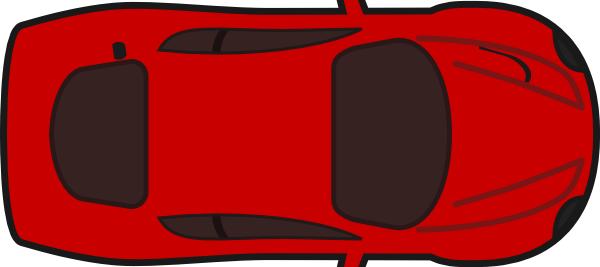
\includegraphics[width=0.6\textwidth]{car_image}
    \caption{An image of a car \label{fig:visualisation_module:car_image} }
\end{figure}

The first thing we need to make sure of is that the image has equal pixel to meter ratio in both its horizontal and vertical components. That is, if the car has a width of 2 meters and the image an height of 100 pixels (remember that the image heigth corresponds to the car width), then if the car length is $x$ meters, the image width should be equal to $x \times \frac{100}{2}$.

This leaves us with the image shown in figure \ref{fig:visualisation_module:car_image_explained_1}. The blue rectangle represents the limits of the image, and is simply shown here for an easier understanding, it is not part of the image. Notice that the image is limited to include only the car, and not any additional empty space.

\begin{figure}[h!]
  \centering
    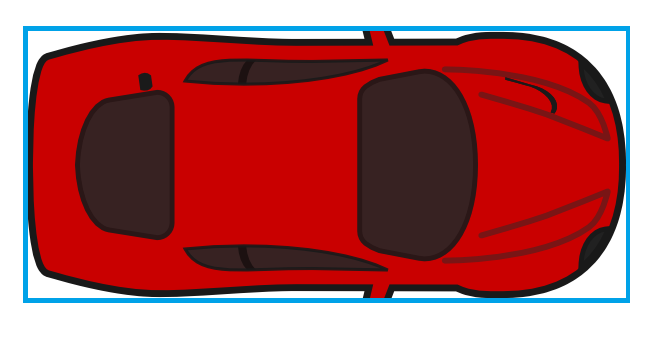
\includegraphics[width=0.6\textwidth]{car_image_explained_1}
    \caption{The car image cropped to the car region \label{fig:visualisation_module:car_image_explained_1} }
\end{figure}

The next step consists in translating the car image such that the center of rotation of the car (usually located in the middle of the rear axle) corresponds to the center of the image. The resulting image would look like the one in figure \ref{fig:visualisation_module:car_image_explained_2}.

\begin{figure}[h!]
  \centering
    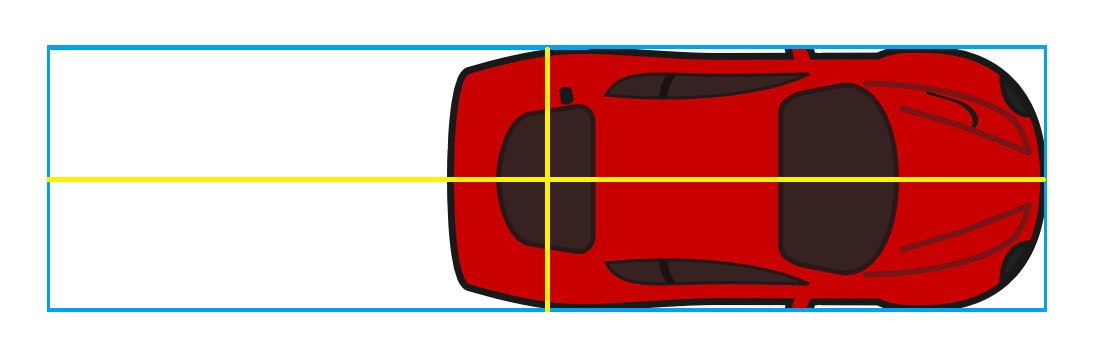
\includegraphics[width=0.9\textwidth]{car_image_explained_2}
    \caption{The car image offsetting the rear axle middle to the center of the image\label{fig:visualisation_module:car_image_explained_2} }
\end{figure}

The yellow lines correspond to the center of the image, like the blue rectangle they are only show for understanding purposes, they are not part of the image. The car rear axle is now located exactly in the center of the image. We make this requirement, since pygame is able to easily rotate images around their center, and as such, if we want to rotate a car, we can simply rotate its image, given that the car rear axle is located in the center of the image.

The final step in the image creation process consists in making it transparent in the pixel regions that do not correspond to the car. Image \ref{fig:visualisation_module:car_image_explained_3}, shows the final car image, with the transparent areas colored in grey. Once again, the grey region is not grey in the car image, but instead is transparent.

Transparency in images can be achieved only by certain image file formats, being \texttt{png} one of them. For creation of these images one can use many image editing programs, the author recommends the free program GIMP \cite{GIMP}.

\begin{figure}[h!]
  \centering
    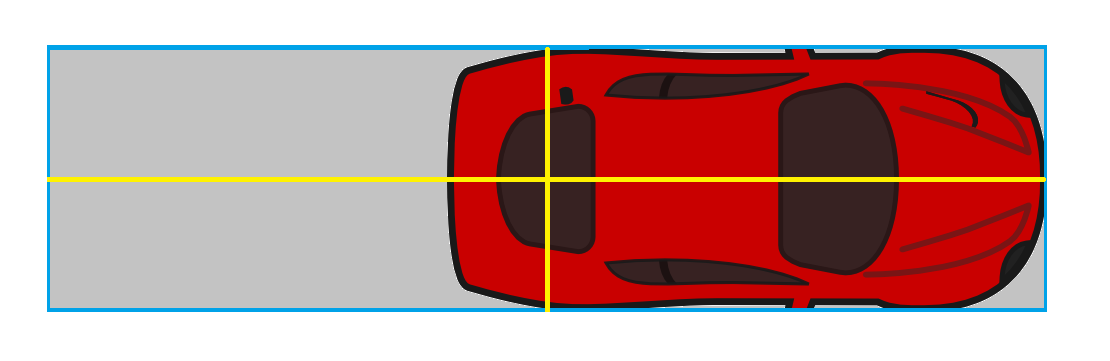
\includegraphics[width=0.9\textwidth]{car_image_explained_3}
    \caption{The car image with transparency in non car areas \label{fig:visualisation_module:car_image_explained_3} }
\end{figure}

\subsubsection{Loading Vehicle Images}

At the initialization of the VisualisationModule class, the vehicle images are loaded. The loading process consists in accessing the image file and loading into memory, and afterwards resize it so that the image has the correct dimensions for the SML World visualisation window.

The image is first loaded using \texttt{pygame.image.load}, and afterwards rescaled using \texttt{pygame.transform.smoothscale}. In order to find the new image size, we simply convert the car width into the corresponding pixel distance in the visualisation window. The ratio between the original image height and the car width in pixels gives us the resizing ratio. This resizing ratio is then applied the original image, both in the height and width dimensions. We now have a car image with a scale appropriate to the visualisation window.

The method implementing this procedure is \texttt{load\_vehicle\_image} in the VisualisationModule class. This method is used by several load functions, like \texttt{load\_red\_car\_image}, \texttt{load\_truck\_image}, \texttt{load\_big\_box\_image} and \texttt{load\_goal\_image}.

\subsubsection{Drawing Vehicles}

To draw a vehicle we need its state $(x,y,\theta)$. The first step consists in rotating the vehicle image, so that it matches the current vehicle $\theta$. This is achieved using \texttt{pygame.transform.rotate}, which returns a new image with the vehicle rotated. Due to the restrictions imposed on the vehicle image creation (see \ref{visualisation_module:creating_vehicle_images}), the center of the rotated image will still correspond to the car rear axle.

We then get the pixel position $(p_x,p_y)$ corresponding to the car position. The rotated image is then placed at $(p_x - \frac{width}{2}, p_y - \frac{height}{2})$. This guarantees that the vehicle's rear axle will be positioned at $(p_x,p_y)$, as desired.

The \texttt{draw\_vehicle\_image} method implements this functionality. This method is called by other methods such as \texttt{draw\_red\_car}, \texttt{draw\_truck}, \texttt{draw\_big\_box} and \texttt{draw\_goal}.

\subsubsection{Drawing Ids}

For many purposes it might be necessary to show the vehicle ids next to the corresponding vehicles. The ids are drawn next to the vehicles if the VisualisationModule's attribute \texttt{show\_ids} is set to \texttt{True}, otherwise they are not.

The id drawing functionality is implemented by the \texttt{draw\_id} method.

\subsubsection{Drawing the next frame}

pygame's image display is based on the \texttt{pygame.Surface.blit} process. \textit{Blitting} consists in drawing one image on top of another.

In order to show the environment and the vehicles in it we first need to blit the environment (background) image onto the Visualisation Window. Afterwards, we need to blit all of the vehicles onto the Visualisation Window, this results in the Visualisation Window displaying the environment and the vehicles in it.

In order to draw a new frame, with vehicles in different places, we need to remove the previously placed vehicles and then draw the new ones. Unfortunately it is impossible to remove the vehicles once they have been blitted onto the visualisation window, so the solution consists in blitting the whole background image once again onto the Visualisation Window, effectively cleaning all of the vehicles. The new vehicles are then blitted once again on top of this clean background image.

When blitting the whole environment image, we are effectively blitting many regions with no vehicles on it. This means that blitting in this regions is useless, since it will simply replace the old pixels with new pixels with the same values. In order to try to remove some of this unecessary, and expensive, blitting, a "smart blitting" is implemented. 

The smart blitting tries to blit only in regions that are indeed necessary to blit. To do so, every time a vehicle is drawn, we store in memory the region where the vehicle was drawn. In the next frame, instead of blitting the whole background, we simply blit the background in the stored regions, corresponding to the places where vehicles are drawn. This results in less areas being blitted, and it was observed that it resulted in less computational expense.

This blitting technique might become more expensive than the whole background blitting if there are a big number of vehicles in the image. To date this was not noticed. But it is the belief of the author that there is the possibility of this happening. The concern is that it might be less expensive to blit one region of $x^2$ pixels, than blitting a big number of regions with a combined area smaller than $x^2$ pixels.

\subsection{Threading restrictions}
\label{visualisation_module:threading_restrictions}

pygame requires the main thread of the program in order to do event handling and render the graphics, this would mean that the VisualisationModule would have to run in the main thread of the SML World.Since we would like to have pygame running on it's own independent thread, the solution found was to use the \texttt{multiprocessing} module to create a new python process which would run the Visualisation Module and give pygame the main thread of this process. This solution was based on the suggestion given in \cite{pygame_threading}.

Since the Visualisation Module is now running on a separate process, it cannot have access to the SML World memory, like the other modules have. However, the Visualisation Module requires only the vehicle states to draw them, and this information can be sent via messages, as explained in the following section.

\subsection{Interfacing with the SML World}

The Visualisation Module needs information about the SML World, namely the vehicles to draw. To get this information, and remembering, that we do not have direct access to the SML World, and the vehicles in it, we set up a UDP connection between the SML World and the Visualisation Module. Currently this communication channel is only one way and it consists in vehicle states being sent from the SML World to the Visualisation Module.

Remembering \ref{fig:visualisation_module_diagram} we know that this communications is made making use of the classes Visualisation Module Sender and Visualisation Module Receiver. 

The Visualisation Module Sender class, is a class that will loop on its own thread, and its task consists in creating and sending the UDP messages containing the vehicle information to the Visualisation Module. This class is instantiated by the SML World, and has a reference to it, being able to interact with the Vehicles Dictionary containing the information about the vehicles.

The class constructor takes as arguments \texttt{visualisation\_address} and \texttt{desired\_rate}. The first corresponds to the IP of the computer running the Visualisation Module, it can be \texttt{\'localhost\'} if the module is running on the same computer, or a standard IP address, if one wishes to have the Visualisation Module running on another computer. \texttt{desired\_rate} defines the frequency at which messages will be sent to the Visualisation Module. 

Similarly to the Sender class, the Visualisation Module Receiver class will also loop on its own thread, however this class is instantiated by the Visualisation Module. The Receiver class is responsible for receiving and parsing the UDP messages sent by the Sender class. The parsed information corresponds to the relevant information about the vehicles present in the SML World.

A typical UDP message exchanged between contains the information about all the vehicles in the SML World. The information about each vehicle consists of the id of the vehicle, the state $(x,y,\theta)$, and the class name. The class name allows us to know which kind of vehicle we are drawing, car, truck or even obstacles. For more details about the format of the exchanged message and the parsing of it, one should look at the implementation details in the class code.

Each UDP message also has a packet number, which is used to compensate for the unreliability of the UDP protocol. Every time a message is sent from the Sender Module, a packet number is added to the message. The packet number starts at 1, and it increases by 1 at each message. This allows the Receiver Module, to know if it is receiving the packets in the correct order, and in case it is not, it will issue a warning via terminal to the user, and ignore said packet.